\documentclass[runningheads]{llncs}

\usepackage[T1]{fontenc}
\usepackage{graphicx}
\usepackage{hyperref}
\usepackage{booktabs}
\usepackage{amsmath}
\usepackage{tikz}
\usetikzlibrary{positioning}
\usepackage{orcidlink}

\begin{document}

\title{GeoProbe: Interactive Attention Intervention for Explainable Image
Geolocation}
\titlerunning{GeoProbe}

\author{Anh-Duy Le\inst{1}\orcidlink{0009-0004-1701-8976} \and
Gia-Huy Tran\inst{1} \and
Duc-Tuan Luu\inst{2}\orcidlink{0000-0003-3893-8582} \and
Anh-Duy Tran\inst{3}\orcidlink{0000-0002-8036-954X} \and
Duc-Tien Dang-Nguyen\inst{4}\orcidlink{0000-0002-2761-2213}}

\authorrunning{A.-D. Le et al.}

\institute{University of Science, VNU-HCM, Ho Chi Minh City, Vietnam\\
\email{\{laduy232,tghuy23\}@clc.fitus.edu.vn}
\and
University of Information Technology, VNU-HCM, Ho Chi Minh City, Vietnam\\
\email{tuanld@uit.edu.vn}
\and
DistriNet, KU Leuven, Leuven, Belgium\\
\email{anh-duy.tran@kuleuven.be}
\and
University of Bergen, Bergen, Norway\\
\email{ductien.dangnguyen@uib.no}}

\maketitle

\begin{abstract}
Worldwide image geolocation models such as GeoCLIP estimate GPS coordinates
from a single photograph, yet they provide no account of which visual evidence
supports a prediction. Post-hoc saliency is correlational: it indicates where
activation concentrates without establishing that the highlighted evidence
causes the output. We present GeoProbe, an interactive system for causal
analysis of image geolocation. Given a region specified manually or obtained
from the prompt-free WeDetect-Uni proposal generator, GeoProbe adds
a key-indexed bias to the pre-softmax attention logits of the CLIP vision
tower, independently per layer. It executes GeoCLIP with and without the
intervention and displays both predictions and their geodesic displacement.
On all $2{,}997$ Img2GPS3k images, we search single and multi-layer
interventions using a discovery split and evaluate the selected configuration
on a held-out split. A three-layer configuration achieves $+11.94$~km under
the clipped mean-improvement score on discovery but $-3.66$~km on holdout
(95\% CI $[-20.43,12.40]$), and does not significantly outperform the
selected single layer. Nevertheless, it moves the predicted coordinate by
$189.5$~km on average while retaining an image-embedding cosine similarity of
$0.9984$. The results position GeoProbe as a tool for measuring causal
sensitivity rather than as an accuracy-improvement mechanism, and demonstrate
the importance of held-out validation when interpreting attention
interventions.

\keywords{Image Geolocation \and Explainability \and Attention Intervention
\and Vision--Language Models.}
\end{abstract}

\section{Introduction}

Estimating the geographic origin of a photograph from its pixels alone has
progressed from retrieval over geotagged collections~\cite{hays2008im2gps},
through classification over discretised geographic
cells~\cite{weyand2016planet,pramanick2022translocator}, to contrastive
alignment between images and continuous GPS coordinates.
GeoCLIP~\cite{cepeda2023geoclip} exemplifies the latter: a
CLIP~\cite{radford2021clip} vision tower is aligned with a location encoder,
and inference reduces to nearest-neighbour retrieval over a gallery of
$10^{5}$ coordinates. Such models are accurate enough to be practically useful
and, for the same reason, consequential --- the capability supports both the
verification of news imagery and the inference of location from photographs
shared without geotags.

Despite this, the evidential basis of an individual prediction remains
largely opaque. It is widely assumed that these models exploit road
markings, vegetation, licence plates and shopfront text, but the supporting
evidence is predominantly anecdotal or derived from attention maps.
Whether raw attention weights explain predictions remains
contested~\cite{jain2019attention,wiegreffe2019attention}. Gradient-based
maps~\cite{selvaraju2017gradcam}, attention rollout~\cite{abnar2020rollout}
and Transformer relevance propagation~\cite{chefer2021transformer} assign
importance to regions, but do not directly test the output under an internal
intervention; saliency methods can also fail basic model- and data-randomisation
checks~\cite{adebayo2018sanity}. Input-space perturbation methods instead mask
pixels~\cite{petsiuk2018rise} or replace image regions~\cite{goyal2019counterfactual},
but may confound model sensitivity with the distribution shift caused by an
altered image. The practical question here is how a prediction changes when a
specific attention pathway is manipulated while pixels and weights stay fixed.
Such analysis is established in language models, where interventions identify
internal routes associated with model behaviour~\cite{vig2020causal,meng2022rome,geva2023dissecting}.
We transfer that approach to image
geolocation and make its geographic effect directly observable.

We present GeoProbe, whose contributions are threefold. First, an
interactive system applying region-conditioned, per-layer attention
intervention to the GeoCLIP vision tower at inference time, requiring
neither training, gradients nor architectural modification, and presenting
the unmodified and intervened predictions jointly on a map. Second, an
object-proposal workflow in which WeDetect-Uni~\cite{fu2026wedetect}
supplies category-agnostic foreground regions without requiring a prompt for
each image, enabling the same intervention to be evaluated at dataset scale.
Third, a quantitative study on Img2GPS3k~\cite{vo2017revisiting} that uses a
discovery/holdout protocol to test single layers and multi-layer
combinations. The study quantifies output sensitivity while showing that
apparently favourable search results need not generalise to unseen images.

\section{System}
\label{sec:system}

\subsection{Background}

GeoCLIP~\cite{cepeda2023geoclip} encodes an image $x$ with a CLIP ViT-L/14
vision tower $f_{\mathrm{img}}$ and GPS coordinates with a location encoder
$f_{\mathrm{loc}}$, then retrieves
\begin{equation*}
\hat{g}(x)=\arg\max_{g\in\mathcal{G}}
\langle\bar f_{\mathrm{img}}(x),\bar f_{\mathrm{loc}}(g)\rangle .
\end{equation*}
Here, $\bar{\cdot}$ denotes $L_2$ normalisation and $\mathcal{G}$ is a fixed
gallery of $10^{5}$ coordinates. GeoProbe leaves $f_{\mathrm{loc}}$ and
$\mathcal{G}$ unmodified throughout; every intervention acts upon
$f_{\mathrm{img}}$ alone, so that any change in $\hat{g}$ is attributable to
the image pathway.

\subsection{Region-Conditioned Attention Intervention}
\label{sec:intervention}

In each of the $L=24$ self-attention layers of the vision tower, attention
weights are obtained as $\mathrm{softmax}(QK^{\top}/\sqrt{d})$ over a
sequence of $257$ tokens: one \texttt{CLS} token followed by $256$ patch
tokens arranged on a $16 \times 16$ grid. Given a region mask
$m \in \{0,1\}^{256}$ indicating the patches falling within the selected
region, GeoProbe adds a key-indexed bias to the attention logits of layer
$\ell$ prior to the softmax,
\begin{equation}
  A^{(\ell)} = \mathrm{softmax}\!\left(
  \frac{QK^{\top}}{\sqrt{d}} + \beta^{(\ell)} \right),
  \qquad
  \beta^{(\ell)}_{j} =
  \begin{cases}
    0      & j = 0 \quad (\texttt{CLS}), \\
    a_\ell & j > 0,\; m_{j-1} = 1, \\
    b_\ell & j > 0,\; m_{j-1} = 0.
  \end{cases}
  \label{eq:bias}
\end{equation}

Three properties make this a suitable analytical primitive. The bias is
indexed by key and broadcast across all queries and heads, so every token
--- including \texttt{CLS} as a query --- draws proportionally more
information from within the region when $a_\ell > 0$ and less from outside
when $b_\ell < 0$. It is exactly a multiplicative reweighting of attention
mass by $\exp(\beta_j)$, so the control may be presented either as a logit
bias or as a scale factor. And $a_\ell = b_\ell = 0$ is an exact no-op, so
the reported baseline is the unmodified model rather than an approximation.
The \texttt{CLS} key is never biased: as a summary token rather than a
spatial patch, the interior/exterior distinction does not apply to it, and
biasing it would confound the regional effect with a global rescaling of the
summary pathway.
Here, ``causal'' refers narrowly to the effect of this controlled operation on
the model's computation; it does not by itself establish that a semantic object
causes the prediction in the photographed world.

\subsection{Mapping Regions to Patches}

A region delineated on the original image cannot be transferred to the patch
grid directly, since CLIP resizes the shorter side to $224$ pixels and then
applies a centre crop. GeoProbe replicates this geometry on the region
coordinates, so that a patch is marked in-region only if it remains so after
preprocessing. Regions falling entirely outside the centre crop yield an
empty mask and therefore an exact no-op. We retain these cases in the
full-dataset results and additionally report the active-mask subset. Multiple
regions are combined by union.

\subsection{Prompt-Free Region Proposals}

Manually delineated rectangles support targeted case studies, but they do
not scale to a complete dataset and make the analysis depend on a
user-supplied concept. For systematic evaluation, GeoProbe uses WeDetect-Uni,
a universal proposal generator trained with a learned objectness prompt to
retrieve category-agnostic foreground boxes~\cite{fu2026wedetect}. It
therefore avoids the per-image text query required by grounded detectors such
as Grounding DINO~\cite{liu2024grounding}. The detector
never observes ground-truth coordinates. Proposals are computed once and
cached; downstream layer searches only change the attention intervention, so
every configuration receives identical regions.

\subsection{Implementation}

A FastAPI backend loads GeoCLIP once at startup and patches the eager
attention forward pass of all $24$ vision layers according to
Eq.~\ref{eq:bias}; a React frontend provides region selection, per-layer
control and map display. One request returns both the unmodified and the
intervened top-$k$ predictions, so the comparison presented to the user is
always between two forward passes of identical weights. Manual rectangles
are used in the live interaction, while cached WeDetect-Uni proposals provide
the reproducible dataset-scale analysis reported below.

\section{Demonstration}
\label{sec:demo}

\begin{figure}[t]
  \centering
  \small
  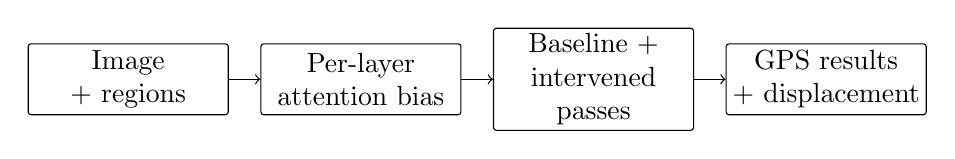
\begin{tikzpicture}[
      node distance=4mm,
      stage/.style={draw, rounded corners=1pt, align=center,
                    minimum height=9mm, text width=24mm, inner sep=2pt},
      arrow/.style={->, line width=0.45pt}]
    \node[stage] (input) {Image\\+ regions};
    \node[stage, right=of input] (control) {Per-layer\\attention bias};
    \node[stage, right=of control] (passes) {Baseline +\\intervened passes};
    \node[stage, right=of passes] (output) {GPS results\\+ displacement};
    \draw[arrow] (input) -- (control);
    \draw[arrow] (control) -- (passes);
    \draw[arrow] (passes) -- (output);
  \end{tikzpicture}
  \caption{Interactive analysis flow. Regions may be drawn manually or loaded
  from WeDetect-Uni; both model outputs are presented together.}
  \label{fig:interaction_flow}
  \vspace{-2mm}
\end{figure}

Attendees operate the system directly through three short scenarios.

\subsubsection{Regional dependence.}
The attendee uploads a street-level image, marks a visual cue such as a sign or
licence plate, and suppresses its region. A large map displacement demonstrates
sensitivity to that evidence; a small displacement indicates that the current
prediction is stable under the intervention.

\subsubsection{Proposal comparison.}
For a benchmark example, cached WeDetect-Uni proposals can be applied
individually or as a union. The resulting displacements distinguish sensitivity
to one foreground object from sensitivity to the broader object-bearing region,
without a text prompt tailored to the image.

\subsubsection{Layer localisation.}
The attendee compares a single active layer with a multi-layer schedule.
Broader intervention often increases displacement without improving error,
mirroring Section~\ref{sec:experiments}. Resetting all biases to zero restores
the baseline exactly.

\subsection{Deployment and Relevance}

The live system stores GeoCLIP, its $10^5$-point GPS gallery, location
embeddings and cached proposals locally. The current interface obtains
basemap tiles and reverse-geocoded place names from public map services;
these provide cartographic context but are not part of model inference.

We bring the demonstration machine; it needs no GPU and runs inference
offline. The appendix states the setup requirements in full. The implementation and
experiment scripts will be made publicly available upon acceptance.
GeoProbe connects multimodal geolocation with causal explanation: rather than
presenting an attention map as evidence, it lets the attendee change an
attention pathway and observe the consequent geographic output. This
distinction is relevant to both multimedia verification and the privacy risks
of inferring location from untagged images.

\section{Quantitative Study}
\label{sec:experiments}

\subsection{Experimental Setup}

We evaluate on all $2{,}997$ Img2GPS3k images~\cite{vo2017revisiting}.
WeDetect-Uni Base generates category-agnostic proposals once for the complete
set. We cache boxes at an objectness threshold of $0.15$ after non-maximum
suppression ($0.7$ IoU), then form the intervention mask from the union of at
most $100$ boxes scoring at least $0.4$. This produces $6{,}152$ boxes in
$2{,}081$ images; $2{,}058$ images retain a non-empty mask after CLIP's centre
crop. Images without an active mask remain in the evaluation as exact no-ops,
so the reported metrics describe the complete benchmark.

For every active layer, the same in-region and out-of-region biases are applied
to all $16$ heads, with base magnitudes $a=+2$ and $b=-2$. We measure top-1
geodesic error and
prediction displacement. For image $i$, improvement is
$\Delta_i=d_i^{\mathrm{base}}-d_i^{\mathrm{int}}$, so positive values are
better. Because a gallery change can move a prediction across continents, the
selection score is the mean of
$\operatorname{clip}(\Delta_i,-2500,2500)$~km. Confidence intervals use
$10{,}000$ paired bootstrap resamples over images.

We deterministically assign $1{,}079$ images to discovery and $1{,}918$ to
holdout by hashing the file name. Model selection uses discovery only. A
preliminary mixed-precision layer sweep on the discovery split supplies five candidates,
$\{2,4,7,12,3\}$, ordered by discovery score. We evaluate all $26$ subsets containing two to five of
these layers under three strength schedules: fixed $2$ per layer,
$2/\sqrt{k}$, and $2/k$, where $k$ is the number of active layers. Together
with five single-layer controls, this gives $78$ combinations and five
controls. The confirmatory pass uses deterministic FP32 with TF32 disabled.

\subsection{Held-Out Results}

The discovery split selects layers $\{2,7,12\}$ with the $2/k$ schedule,
equivalent to magnitude $0.667$ at each layer. Table~\ref{tab:main} compares
this configuration with the discovery-selected single-layer control. The
apparent discovery gain does not transfer: the selected combination changes
from $+11.94$~km on discovery to $-3.66$~km on holdout. Its paired advantage
over layer 2 is only $0.64$~km (95\% CI $[-16.83,17.57]$). The experiment
therefore does not support synergy between individually promising layers.

\begin{table}[t]
\centering
\caption{Deterministic FP32 results. $\Delta_c$ is mean improvement clipped to
$\pm2500$~km; positive is better. Columns after the discovery score are holdout
metrics. Every column but the last is in kilometres.}
\label{tab:main}
\small
\setlength{\tabcolsep}{2.5pt}
\begin{tabular}{l|rrrrrr}
\toprule
\textbf{Configuration} &
\textbf{Disc. $\Delta_c$} & \textbf{Error} & \textbf{Hold. $\Delta_c$} &
\textbf{95\% CI} & \textbf{Shift} & \textbf{Cosine} \\
\midrule
GeoCLIP baseline & 0.00 & 1716.31 & 0.00 & --- & 0.00 & 1.0000 \\
Layer 2 & +4.95 & 1731.44 & -4.30 & $[-18.83,9.96]$ & 136.15 & 0.9993 \\
Layers 2, 7, 12 ($2/k$) & +11.94 & 1728.86 & -3.66 & $[-20.43,12.40]$ & 189.53 & 0.9984 \\
\bottomrule
\end{tabular}
\end{table}

Despite the absence of an accuracy gain, the intervention exposes output
sensitivity. The selected configuration preserves a mean cosine similarity of
$0.9984$ to the baseline image embedding, yet moves the predicted coordinate
by $189.5$~km on average. GeoCLIP retrieves from $10^5$ location embeddings;
small movements in representation space can therefore cross a gallery
decision boundary and produce a geographically large change.

Increasing the number of layers does not help on average. With fixed magnitude
$2$, mean holdout $\Delta_c$ declines from $-8.22$~km for two layers to
$-39.35$~km for five. The $2/k$ schedule limits this accumulation ($-2.01$ to
$-0.13$~km across sizes) without yielding a consistent positive effect. Candidate rankings also transfer
weakly from discovery to holdout ($r=0.259$), underscoring the risk of
reporting the best result on the same images used to find it.

This conclusion is not an artefact of diluting the result with no-op images.
On the $1{,}321$ holdout images with an active mask, the selected configuration
obtains $-5.32$~km (95\% CI $[-28.75,18.02]$), and its paired advantage over
layer 2 remains only $0.92$~km (95\% CI $[-23.66,25.66]$).

A natural objection is that displacement merely tracks how much of the image
the mask covers. It does not. Over the $2{,}051$ active-mask images of the
all-layer $a=2$, $b=-2$ run, coverage and displacement are negatively related
(Spearman $\rho=-0.256$): the least-covered quartile moves the prediction by a
median of $407$~km with $13.8\%$ of images unmoved, whereas the quartile
covering more than $81\%$ of patches moves it by a median of $0$~km with
$49.4\%$ unmoved. Eq.~\ref{eq:bias} predicts this: a mask spanning nearly
every patch biases every patch key almost equally, and softmax is invariant to
a constant shift. The experiment still isolates
layer-combination effects rather than showing that WeDetect regions are more
informative than arbitrary ones; that claim needs an area-matched random-mask
control.

\section{Conclusion}

GeoProbe makes geolocation evidence amenable to intervention rather than
inspection. Its per-layer pre-softmax bias reads a causal analysis of a
selected region from geographic displacement. On Img2GPS3k, the
discovery-selected multi-layer schedule neither improved held-out error nor
significantly outperformed one layer, yet moved predictions by $189.5$~km at
feature cosine $0.9984$. Sensitivity is therefore an explanatory measurement,
not evidence of improved prediction. Future work will select clue concepts by their
causal effect rather than by detection confidence, and validate the selection
on a fresh benchmark.


\clearpage
\bibliographystyle{splncs04}
\bibliography{reference}

\clearpage
\section*{Appendix: Demonstration Details}

\subsubsection*{Demonstration video.}
A screen capture of the three scenarios of Section~\ref{sec:demo}, recorded on
a live instance and under three minutes long, is available at
\url{https://drive.google.com/drive/folders/1QsH8qOV5hxGi62qoXuWCsY0u6fgqQdQL}.

\subsubsection*{What the live demonstration shows.}
Attendees operate a running instance themselves, on provided samples or their
own photographs. A session lasts two to three minutes: upload an image, obtain
the unmodified prediction, mark a region by hand or load prompt-free
WeDetect-Uni proposals, choose which of the $24$ layers the bias acts on, and
read both predictions and their geodesic separation from the map.

\subsubsection*{Interaction details.}
Regions are drawn as rectangles or selected from returned proposals, and
combine by union. Each layer exposes the in-region bias $a$ and out-of-region
bias $b$, shown as a logit bias or the equivalent attention scale. Setting
every bias to zero is an exact no-op, so the attendee can recover the
unmodified model and verify the displayed baseline. A separate control
evaluates each proposal independently, ranking the regions of one image by the
displacement each induces.

\subsubsection*{Setup requirements.}
We provide the demonstration machine: a laptop holding the $1.6$~GB CLIP
ViT-L/14 checkpoint, the $410$~MB WeDetect-Uni proposal graph, the GPS gallery
and the location embeddings. No GPU is required --- on CPU alone one request
returns both predictions in about eight seconds, and proposal generation takes
about two seconds. Inference runs offline; only basemap tiles and place names
come from public map services, and predictions and displacements stay legible
without them. From the organisers we need table space, mains power and, where
available, an external monitor.

\subsubsection*{Search details.}
Every subset of size two to five of layers $\{2,4,7,12,3\}$, at fixed,
square-root-normalised and linearly normalised strength: $78$ combinations plus
five single-layer controls. Seed $42$, deterministic FP32 with TF32 disabled,
$1{,}081.9$~s on an NVIDIA RTX PRO 6000 Blackwell.


\end{document}
